
\section{Benchmark auf Basis von Interrupts}
\label{chap:benchmark_basis_interrupts}

% A system call is a request in a Unix-like operating
% system made via a software interrupt by 
% Found on http://www.linfo.org/software_interrupt.html


Der Aufbau der Messmethode basiert auf Softwareinterrupts. Dafür wurde ein eigener Kernelmodul erstellt, der den Benchmark beinhaltet und auf verlangen ausführt.
\par
Ein Interrupt erzwingt den Linux Kernel vom Benutzermodus in den Kernelmodus zu wechseln\cite{Mandl2010_3}. Beim Wechsel werden alle laufende Prozesse zwischen gespeichert, angehalten und anschliessend wird eine Interrupt-Service-Routine (ISR) aufgerufen. Genau diese Eigenschaft wird für den Aufbau der Messmethode verwendet. Den während der Ausführung des ISR sind alle Prozesse angehalten und können der Benchmark der sich selbst in der ISR befindet nicht unterbrechen. Somit wird sicher gestellt das nur der Benchmark ausgeführt und die volle Ressourcen des CPU bekommt bis er fertig ist.
\par
Interrupts sind dafür gemacht, damit sie sofort verarbeitet werden. Ein kleines Beispiel soll dies veranschaulichen. Der Benutzer eines Computer drückt eine Taste auf der Tastatur. Dadurch produziert er ein Hardware-Interrupt. Der aktuelle Prozess wird gespeichert und angehalten. Der Kernel stellt über eine Vektor-Tabelle fest um welchen Interrupt es sich handelt und führt die passende ISR aus, die zur Verarbeitung der gedrückte Tasten dient. ISR sind sehr kurze Programmcodes (Microcode). In diesem Fall speichert der Programmcode die gedrückte Taste in den RAM und übergibt die Ressourcen wieder frei. Der letzte Prozess wird danach, falls er nicht bereits fertig war, weitergeführt. Die Interrupts sind nötig um die Daten am Zeitpunkt des Geschehens zu verarbeiten.
\par
\autoref{fig:Interrupt} beschreibt die unterschiedlichen Interrupts und der Ablauf nach einem eingehender Interrupt. Die Hardware-Interrupts\footnote{Je nach Literatur, Sprache oder Betriebssystem werden unterschiedliche Fachausdrücke verwendet. Der Kontext bleibt aber der selbe.} wurden bereits oben beschrieben. Die "Exception / Trap" sind Interrupts die der CPU selber produziert. Als Beispiel für ein solches Interrupt wäre "Divisions by Zero", wenn man probiert eine Zahl durch Null zu teilen. Die Messmethode in dieser Arbeit stützt sich auf die Software-Interrupts. Software-Interrupts werden als Systemcall bezeichnet, die häufig verwendet werden um durch ein Kontextwechsel eine Aufgabe dem Kernel zu übergeben. Durch den Kontextwechsel wird vom unprivilegierten Ring  (Benutzermodus) in den privilegierten Ring (Kernelmodus) gewechselt. Dadurch können auf Befehlssätze und Speicheradressen zugegriffen die im Benutzermodus nicht möglich wären ohne unsicheren Code ausführen zu müssen. Systemcall werden als ISR im selben Kontext ausgeführt wie Interrupts.

\begin{figure}[H]
\centering
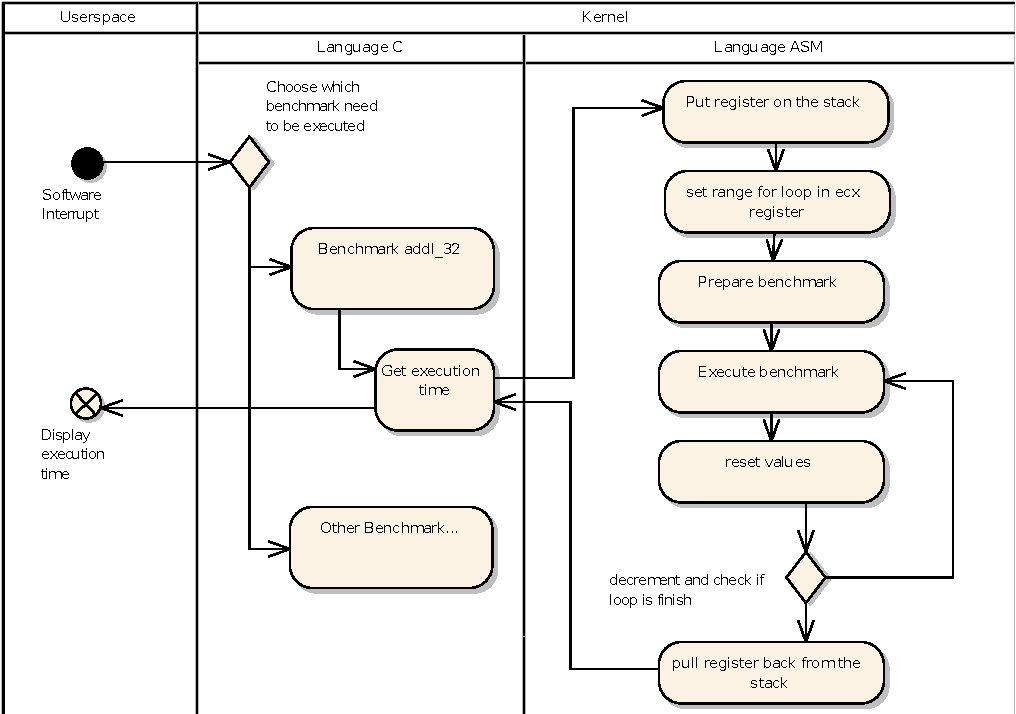
\includegraphics[width=1.0\textwidth]{images/interrupt_ea.pdf}
\caption{Interrupt}
\label{fig:Interrupt}
\end{figure}

\section{Starten des Benchmark über procfs}

Der Benchmark wurde in Form eines Kernelmodul für ein Linux Betriebssystem gebaut. Das Kernelmodul registriert für jeden Benchmark ein Pseudofile, das unter der Verzeichnisstruktur \texttt{/proc/benchmark/} abrufbar ist.
\par
Das \texttt{procfs} oder \texttt{proc filesystem} genannter Filesystem erstellt eine Schnittstelle zwischen dem Benutzermodus und dem Kernelmodus. Es ist ein virtuelles Filesystem, dass unter der Verzeichnisstruktur \texttt{/proc} gemountet wurde\cite{mauerer2010professional}. Die Dateien die sich darin befinden sind Pseudofiles. Sie sind virtuelle, weil sie nicht wirklich existieren und somit auch nicht auf ein Medium gespeichert sind. Beim schreiben beziehungsweise lesen werden die Information am Kernel weiter gegeben, verarbeitet und zurück zum lesen gestellt. Weil das verhalten der Schnittstelle einer Datei entspricht, können für die Lese- und Schreiboperation, die Linux Standart-Werkzeuge verwendet werden.

\lstset{language=Bash}
\begin{lstlisting}
sriolo@desktop ~ $ cat /proc/uptime 
571433.06 1229766.89
\end{lstlisting}
\begin{lstlisting}
sriolo@desktop ~ $ echo 1 > /proc/sys/net/ipv4/conf/default/forwarding
\end{lstlisting}

Im ersten Beispiel wird aus der Datei \texttt{uptime} gelesen, die Betriebszeit kommt als Ausgabe. Das folgende zweite Beispiel zeigt wie in einer Datei geschrieben werden kann. Dabei wird Kernel mitgeteilt dass, er das IP-Forwarding einschalten soll. Ein ähnlicher Aufbau hat das \texttt{sys filesystem}. Die Kommunikation ist dabei schwieriger weil das Design nicht für Menschen lesbar ist, sondern für Programme im Benutzermodus. Im Gegensatz dazu kann das \texttt{procfs} mit den Standard-Werkzeuge im ASCII-Format gelesen und geschrieben werden.
\par
Das \texttt{procfs} ist an dieser Stelle wichtig, weil der Benchmark im Kernelmodus laufen muss. Durch den Befehl \texttt{cat} auf die entsprechende Datei des Benchmark, startet im Kernelmodus den Ablauf für die Messung und gibt die verwendete Zeit als Ausgabe an. Das folgende Beispiel zeigt wie der Benchmark gestartet wird und der CPU durch eine Addieroperation ausgelastet wird.

\begin{lstlisting}
root@galileo ~ $ cat /proc/benchmark/addl_32
321
\end{lstlisting}


\section{Aufbau der Software für die Messung}


\subsection{Grundaufbau und Ablauf eines Benchmark}
Der Grundbau der Software wurde mit der Programmiersprache C geschrieben. Der Kern des Benchmark besteht aus wenige Assembler Befehlssätze. Der Kernelmodul beinhaltet alle in dieser Arbeit relevante Benchmarks. Die \autoref{fig:Benchmark} zeigt der Ablauf des Programm. Durch ein Systemcall, dass über das \texttt{procfs} ausgelöst wird, wird der Benchmark gestartet. Da sich in der Software mehrere Benchmark befinden muss zuerst der Benchmark ermittelt werden. An dieser Stelle werden durch die Funktion \texttt{local\_irq\_save} alle weitere Interrupts geblockt. Die Startzeit wird ermittelt und zwischen gespeichert. Das Programm wechselt zum eigentlichen Benchmark der in Assembler geschrieben ist.


\lstset{language=[x64]Assembler}
\begin{lstlisting}

benchmark_imull_zero:
  stmfd    sp!, {r0-r5}
  ldr r1, = 2147483648
  ldr r3, = 0x0
  ldr r4, = 0x0
loop_benchmark_imull_zero:
  mul r5, r3, r4
  sub r1, r1, #1
  cmp r1, #0
  bge loop_benchmark_imull_zero
  ldmfd    sp!, {r0-r5}
  bx  lr
\end{lstlisting}



\begin{figure}[H]
\centering
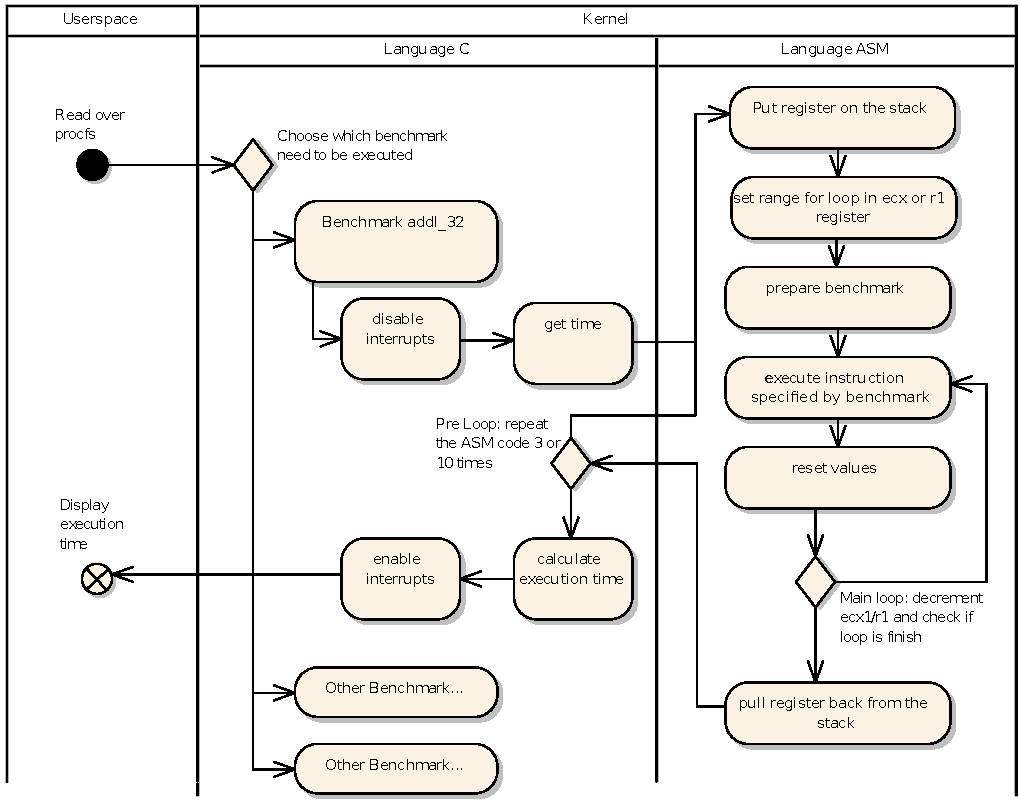
\includegraphics[width=1.0\textwidth]{images/benchmark_ea.pdf}
\caption{Benchmark}
\label{fig:Benchmark}
\end{figure}

\subsection{Kompilation und Programmstruktur}


